\documentclass{beamer}

\usetheme{Berlin}
\usecolortheme{rose}

% \usepackage{amsmath}
% \usepackage{amsthm}
\usepackage{graphicx,epstopdf}
\theoremstyle{plain}
\newtheorem{thm}{Theorem}


\title{Beamer Finale}
\subtitle{Practice}
\author{Kongsak Tipakornrojanakit}
\institute{Mahidol University, International College}
\begin{document}

\begin{frame}
\titlepage
\end{frame}

\begin{frame}
\frametitle{Table of Contents}
\tableofcontents[currentsection]
\end{frame}

\section{Text Colors}
\begin{frame}
\frametitle{Text Colors}
Watch this slide grow.

\begin{itemize}
\item<2-> \textcolor{pink}{Hello, World!}
\item<3-> \textcolor{red}{Hello, Mar!}
\item<4-> \textcolor{blue}{Hello, Alpha Centauri!}
\end{itemize}

\end{frame}

\section{Overlays (Again)}
\begin{frame}
\frametitle{Table of Contents}
\tableofcontents[currentsection]
\end{frame}

\begin{frame}
\frametitle{Overlays (Again)}
Which president said, Most folks are about as happy as they make up their minds to be?

\begin{enumerate}[A]
\item<2-5> James Madison
\item<3-5> Harry Truman
\item<4-6> \textcolor<6>{red}{Abraham Lincoln} 
\item<5-5> Calvin Coolidge
\end{enumerate}

\onslide<1-5> Hint: \\
\onslide<2-5> James Madison ate broccoli.\\
\onslide<3-5> Harry Truman drank milk.\\
\onslide<4-5> Abe Lincoln raised bees.\\
\onslide<5-5> And Cal Coolidge grew silk.
\end{frame}

\section{Figure}
\begin{frame}
\frametitle{Table of Contents}
\tableofcontents[currentsection]
\end{frame}


\begin{frame}
\frametitle{How to add figure}

\begin{columns}
\column{0.5\textwidth}
\begin{figure}
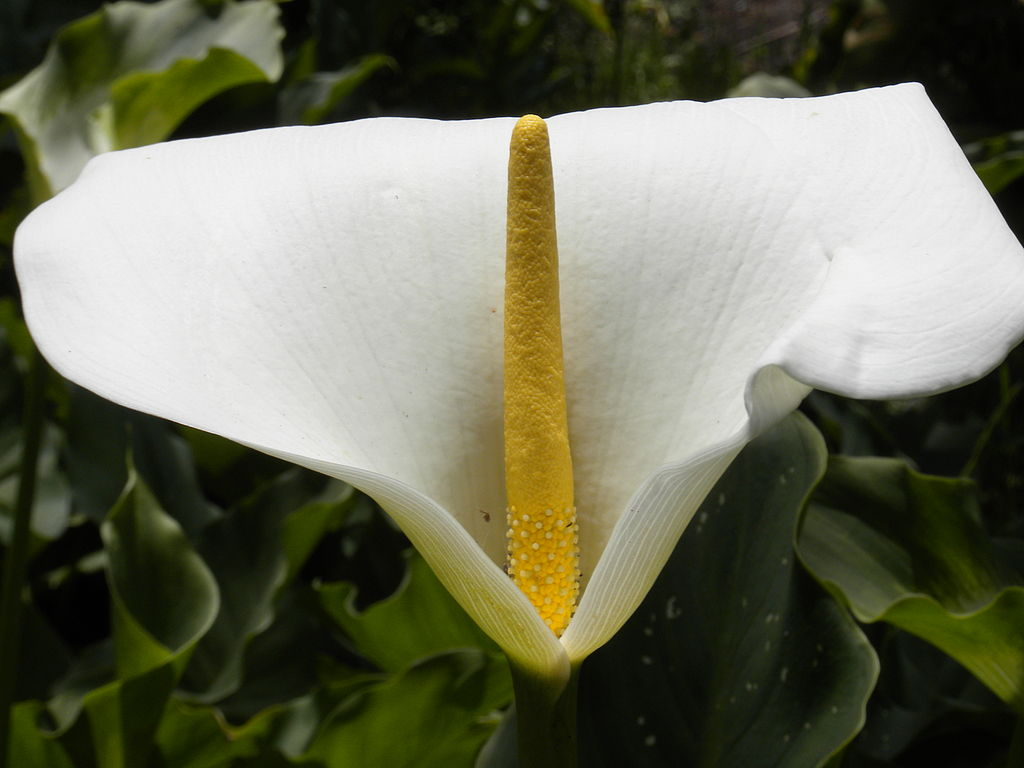
\includegraphics[scale=0.4]{Flower}
\caption{Beautiful flower}
\end{figure}

\pause

\column{0.5\textwidth}
\begin{block}{Observation 1}
Bangkok is a big city.
\end{block}

\pause

\begin{block}{Observation 2}
Salaya is quite nice.
\end{block}

\pause

\begin{block}{Conclusion}
Pad thai is delicious.
\end{block}

\end{columns}
\end{frame}

\section{Mathematical Theorem}
\begin{frame}
\frametitle{Table of Contents}
\tableofcontents[currentsection]
\end{frame}

\begin{frame}
\frametitle{Some Theorem}
\begin{theorem}
$$
\det(M) = \det
\left(
\begin{array}{cc}
M_1 & M_2 \\
M_3 & M_4 \\
\end{array}
\right)
= \det(M_1)\det(M_4 - M_3M_1^{-1}M_2).
$$
\end{theorem}

\begin{Proof}
The proof is not too hard. Try it yourself!
\end{Proof}

\begin{block}
This theorem is called the block matrix identity.
\end{block}
\end{frame}


\section{Table}
\begin{frame}
\frametitle{Table of Contents}
\tableofcontents[currentsection]
\end{frame}
\end{document} 